%简谐振子受迫运动的简单数值计算

\pentry{简谐振子受迫运动\upref{SHOfF}, 微分近似\upref{Diff}, Matlab 编程基础\upref{Matlab}}

以下以弹簧振子的受迫运动为例,介绍一种解 $n$ 阶微分方程的简单方法,以便了解数值解微分方程的基本思想. 但是这种方法误差较大,需要大量计算才能获得较精确的数值解. 在实际运用中已有更复杂更成熟的算法(参考MATLAB常微分方程(组)数值解简介%未完成:词条
).

在简谐振子受迫运动\upref{SHOfF}中,列出的二阶微分方程为
\begin{equation}\label{SHOFN_eq1}
m\ddot y = \alpha \dot y - ky + f(t)
\end{equation}
若已知初值条件(可代入任意具体数值) $\dot y(0) = v_0$,  $y(0) = y_0$, 且已知驱动力 $f(t)$, 此时可以把初值条件代入\autoref{SHOFN_eq1} 求出 $t = 0$ 时的加速度.
\begin{equation}
\ddot y(0) = [- \alpha \dot y(0) - ky(0) + f(0)]/m
\end{equation}
接下来的一小段微小的时间 $\Delta t$ 内( $\Delta t$ 称为\bb{步长},步长越小误差越小), 根据微分近似,可以算出 $t = \Delta t$ 时刻的状态.
\begin{gather}
y(\Delta t) =  y(0) + \Delta y \approx y(0) + \dot y(0) \Delta t\\
\dot y(\Delta t) = \dot y(0) + \Delta \dot y \approx \dot y(0) + \ddot y(0) \Delta t
\end{gather}
微分近似在这里的物理意义是在 $\Delta t$ 内速度和加速度都近似为常数. 把 $y(\Delta t)$ 和 $\dot y(\Delta t)$ 再次代入\autoref{SHOFN_eq1}
\begin{equation}
\ddot y(\Delta t) = [- \alpha \dot y(\Delta t) - ky(\Delta t) + f(\Delta t)]/m
\end{equation}
再次使用微分近似有
\begin{gather}
y(2\Delta t) =  y(\Delta t) + \Delta y \approx y(\Delta t) + \dot y(\Delta t) \Delta t\\
\dot y(2\Delta t) = \dot y(\Delta t) + \Delta \dot y \approx \dot y(\Delta t) + \ddot y(\Delta t) \Delta t
\end{gather}
重复以上各步骤,就可以继续得到 $y(3\Delta t)$,  $y(4\Delta t)$ 等的近似值. 在 $y$-$t$ 图中把这些散点连接起来,就得到了 $y(t)$ 的函数图.

\subsubsection{SHOf.m}
\Matlab
% 参数设定
m = 0.1; % 质量
k = 1; % 劲度系数
a = 0.03; % 阻尼系数
T = 20; % 停止时间
Nstep = 10000; % 步数
A = 2; w = 3; % f(t)=A*sin(w*t);

dt = T/Nstep; % 计算步长
y2 = zeros(step,1); y1 = y2; y = y2; % 矩阵预赋值
y(1) = 0; y1(1) = 0; % 初值, y1 是 y 的一阶导数

% 迭代循环
for ii = 2:step
    y2(ii) = (-a*y1(ii)-k*y(ii)+2*sin(w*(ii*dt)))/m; % 代入微分方程求出 y''.
    y(ii) = y(ii-1) + y1(ii-1)*dt; % y 的微分近似
    y1(ii) = y1(ii-1) + y2(ii-1)*dt; % y' 的微分近似
end

% 画图
t=(0:step-1)*dt;
plot(t,y);
\end{lstlisting}
运行结果如\autoref{SHOFN_fig1},可见开始时驱动力不断给弹簧振子补充能量,振幅变大. 当补充的功率等于消耗的功率时,弹簧做稳定振动.
\begin{figure}[ht]
\centering
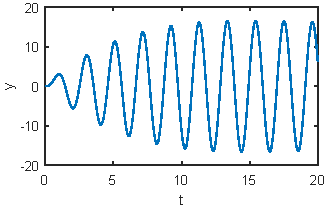
\includegraphics[width=10cm]{./figures/SHOFN.pdf}
\caption{运行结果}\label{SHOFN_fig1}
\end{figure}











